\chapter{Cost Breakdown}\label{ch:cost-breakdown}
If this web app was to be deployed to the public, or be expanded to a larger market, it would be important to
gather estimated costs for hosting the app in the cloud with all the AWS services being used.
The AWS Pricing Calculator can be used to calculate current costs and predict future costs.
To calculate these costs, it is required to specify every implemented feature and several projected inputs and outputs,
such as amount of data transferred on the app per month~\parencite{amazon2022aws}.
The monthly cost and a yearly cost of deploying the app in its current state was calculated first, with an estimated
user-base of 100.
Following this, the calculator was used to predict monthly and yearly costs for scaling the deployment up to larger
user-bases.
These figures were calculated for scaling the app up to 10,000 users, one million users, and ten million users, which
would require upgrading some selected AWS features.

Figure~\ref{fig:100-users} details the monthly and yearly cost of running the current AWS configuration for 100 users.
With this configuration, the cost of maintaining the web app would be 112.55 USD per month or 1,350.60 USD per year,
with the largest costs being RDS, VPC, and ELB\@.

\begin{figure}[!htbp]
    \centering
    \subfloat{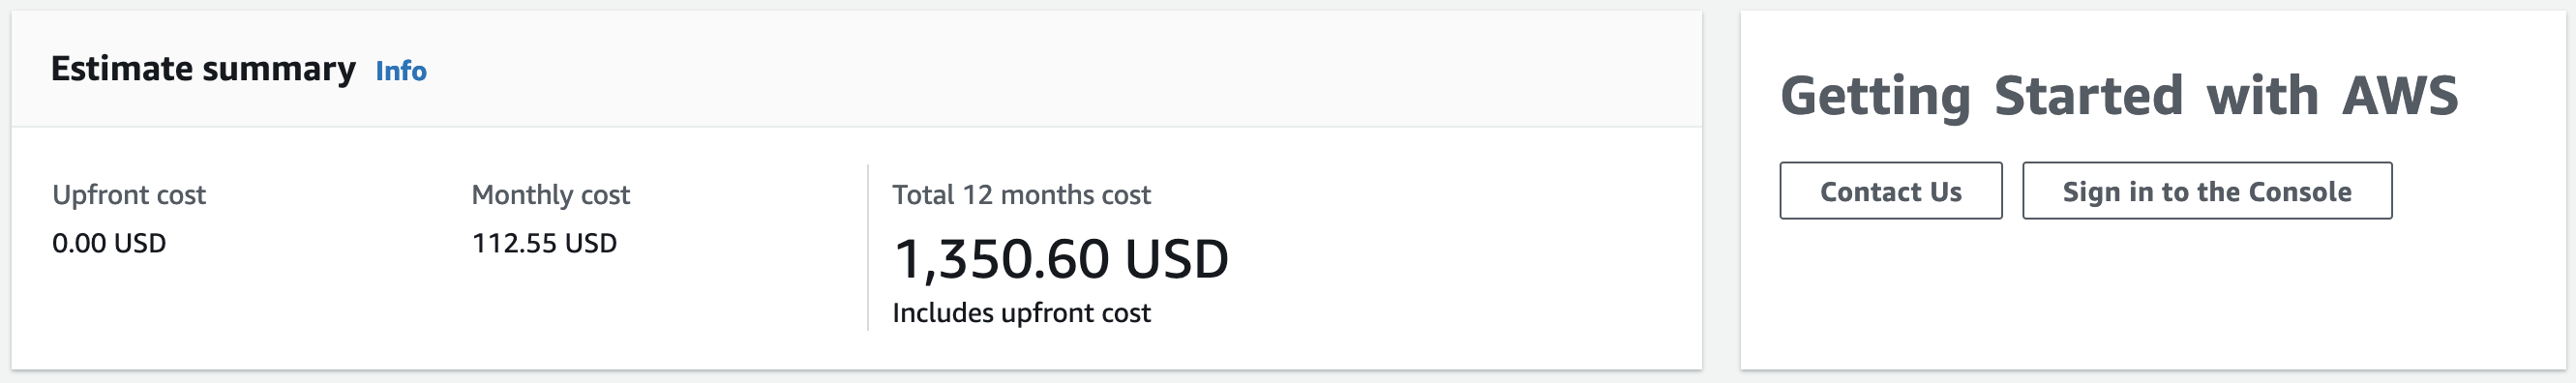
\includegraphics[width=150mm]{resources/cost/estimated-costs-1}}\hfill
    \subfloat{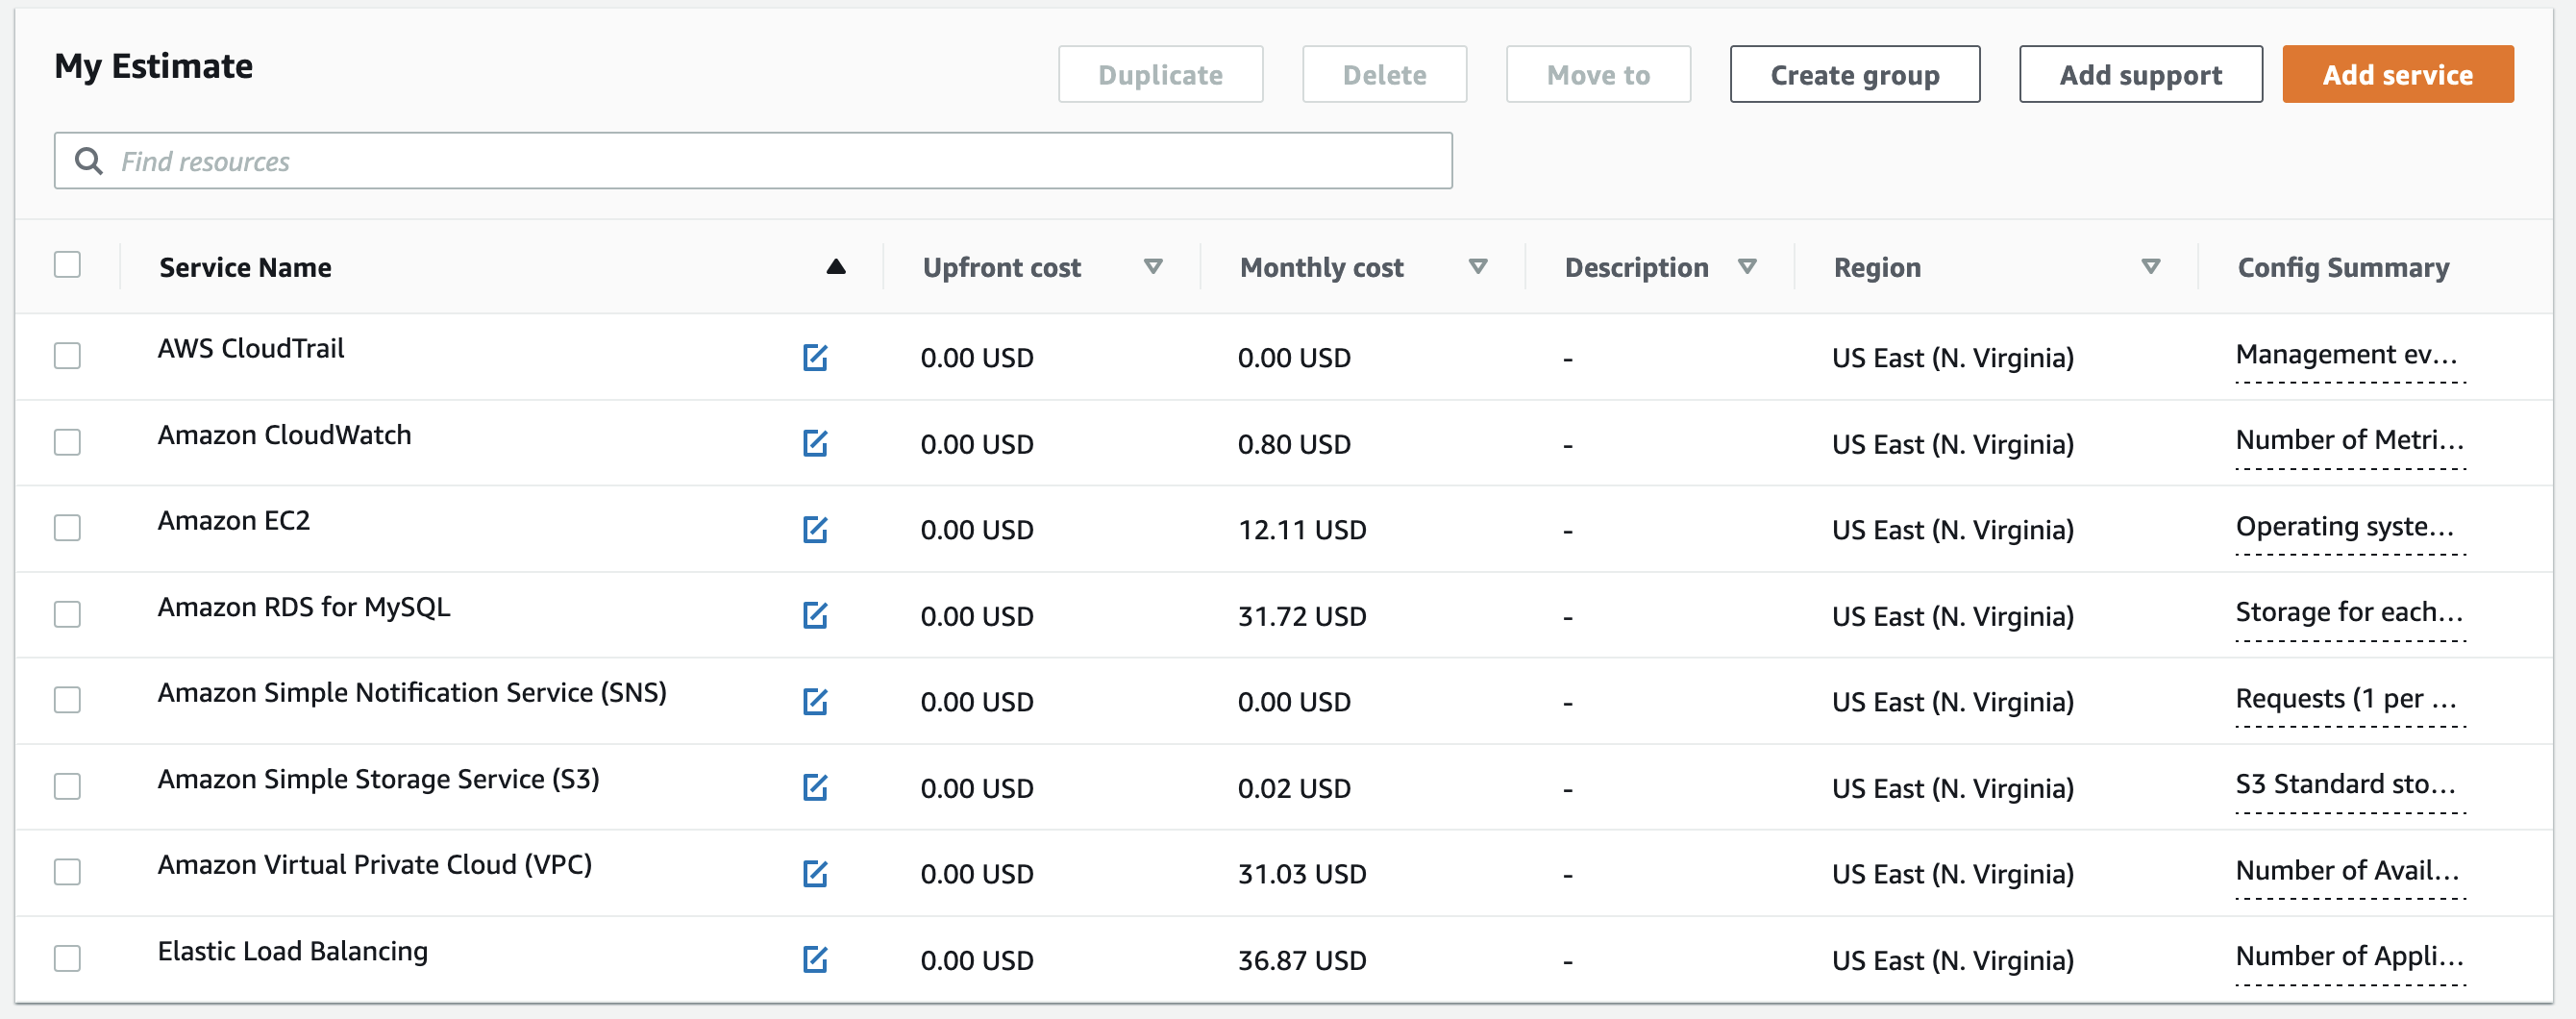
\includegraphics[width=150mm]{resources/cost/estimated-costs-2}}
    \caption{Estimated cost with current configuration for 100 users.}
    \label{fig:100-users}
\end{figure}


\clearpage
\section{Scaling Up to 10,000 Users}\label{sec:scaling-up-to-10000-users}
A vertical scaling approach was taken to scaling the application deployment up to 10,000 users.
Vertical scaling refers to increasing the instance size.
The only two services which are required to be scaled up to accomplish this are EC2 and RDS, due to the increase
in users and demand.
For EC2, an additional three instances were added, and all instances were scaled up to the \mintline{zsh}|t2.medium|
instance type, which provides 4 GB of RAM each.
This gives the web app a total memory of 20 GB of RAM, which is enough to comfortably handle the expected
increase in users accessing the web app.
The RDS storage was also increased from 30 GB to 70 GB as more information, in the form of user and story records,
will be stored in the database.
This scaling would increase the cost of maintaining the web app to 222.03 USD per month or 2,664.41 USD per year.

\begin{figure}[!htbp]
    \centering
    \subfloat{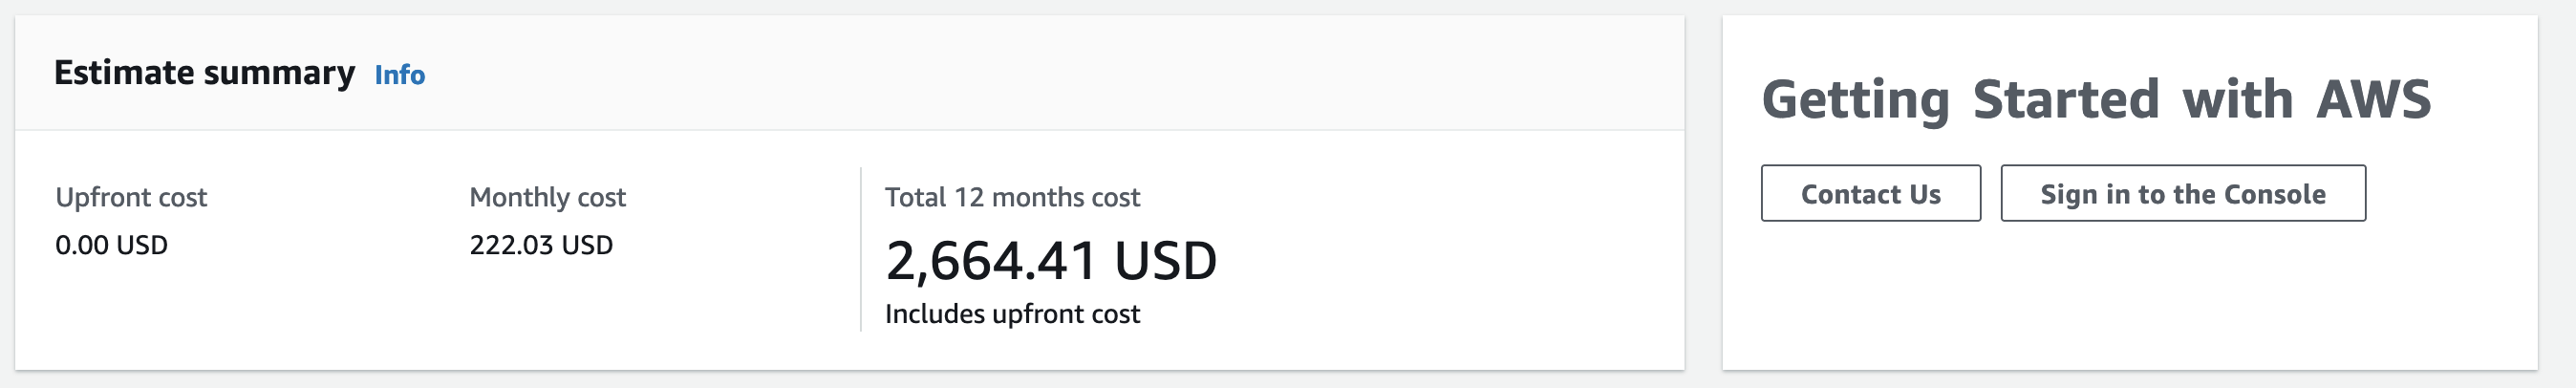
\includegraphics[width=150mm]{resources/cost/scaling-10,000-1}}\hfill
    \subfloat{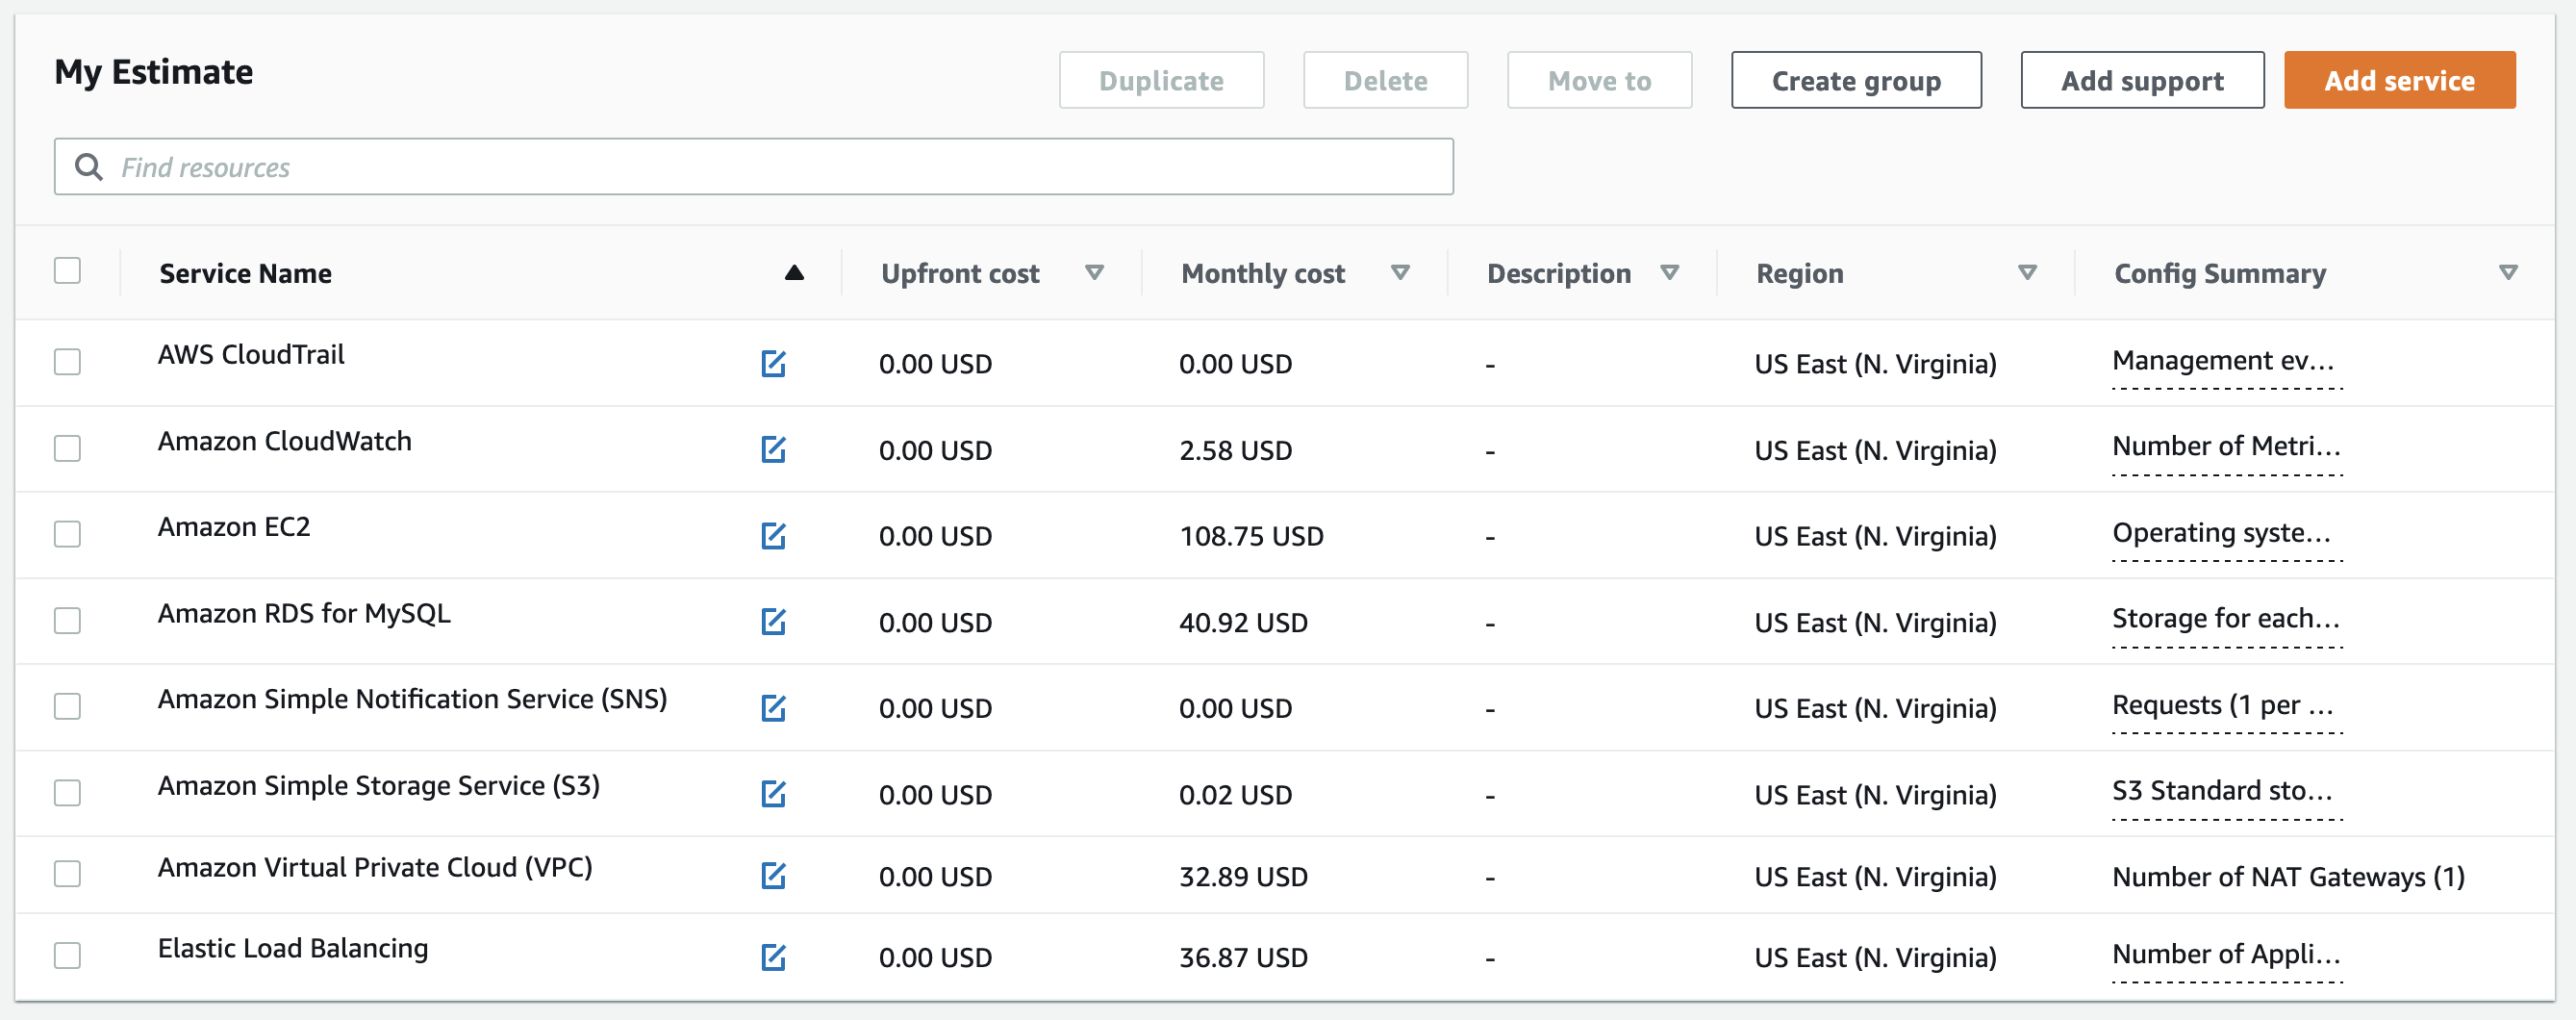
\includegraphics[width=150mm]{resources/cost/scaling-10,000-2}}
    \caption{Estimated cost for scaling up to 10,000 users.}
    \label{fig:10,000-users}
\end{figure}

\clearpage
\section{Scaling Up to 1 Million Users}\label{sec:scaling-up-to-1-million-users}
A similar approach was taken when scaling the application up to 1 million users.
The total number of EC2 instances was doubled and the instance type for each was changed to
\mintinline{zsh}|t3.xlarge|.
At 16 GB of memory per instance, a total of 160 GB of memory is available.
For scaling up to 1 million users, the RDS instance type was changed to \mintline{zsh}|db.t3.medium|.
This gives the database an additional 3 GB of memory, making it able to handle more concurrent
requests from a larger number of users.
The total RDS storage was increased by a further 20 GB, making a total of 100 GB of storage.
This scaling would increase the cost of maintaining the web app to 965.03 USD per month or 11,568.41 USD per year.

\begin{figure}[!htbp]
    \centering
    \subfloat{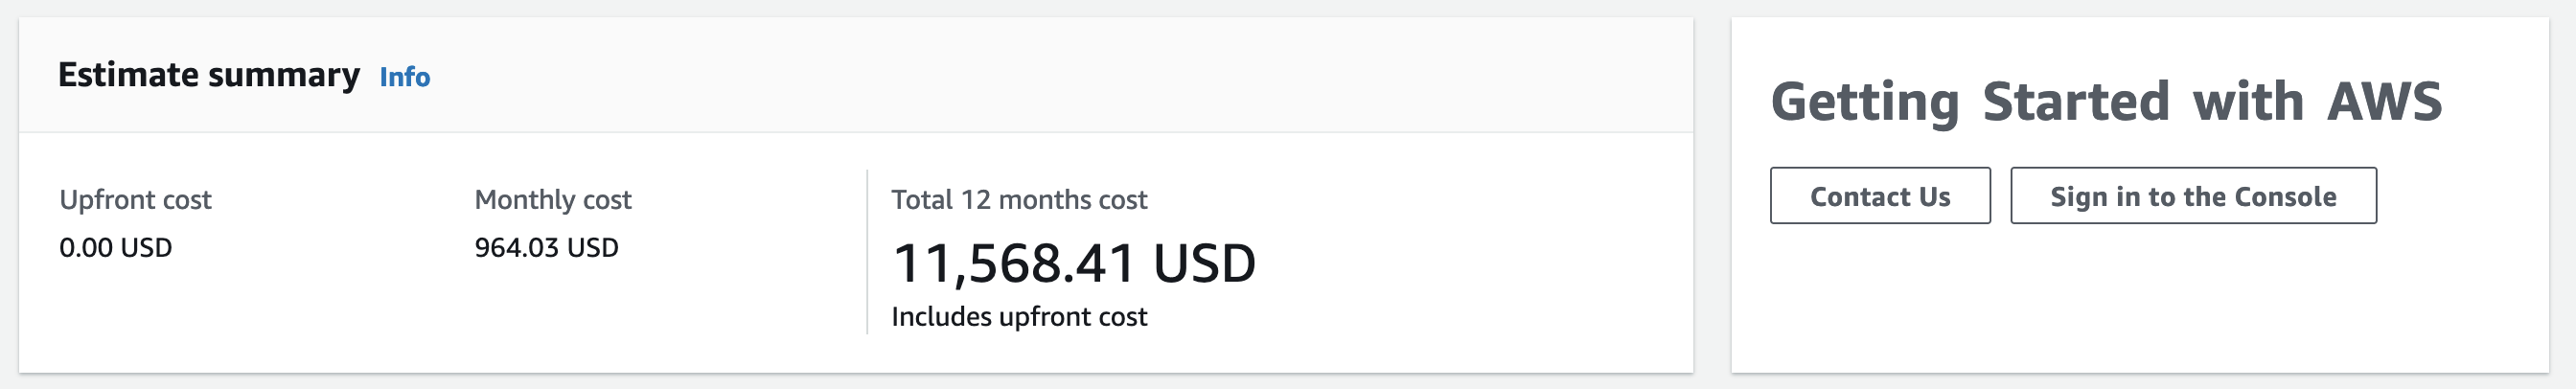
\includegraphics[width=150mm]{resources/cost/scaling-1-million-1}}\hfill
    \subfloat{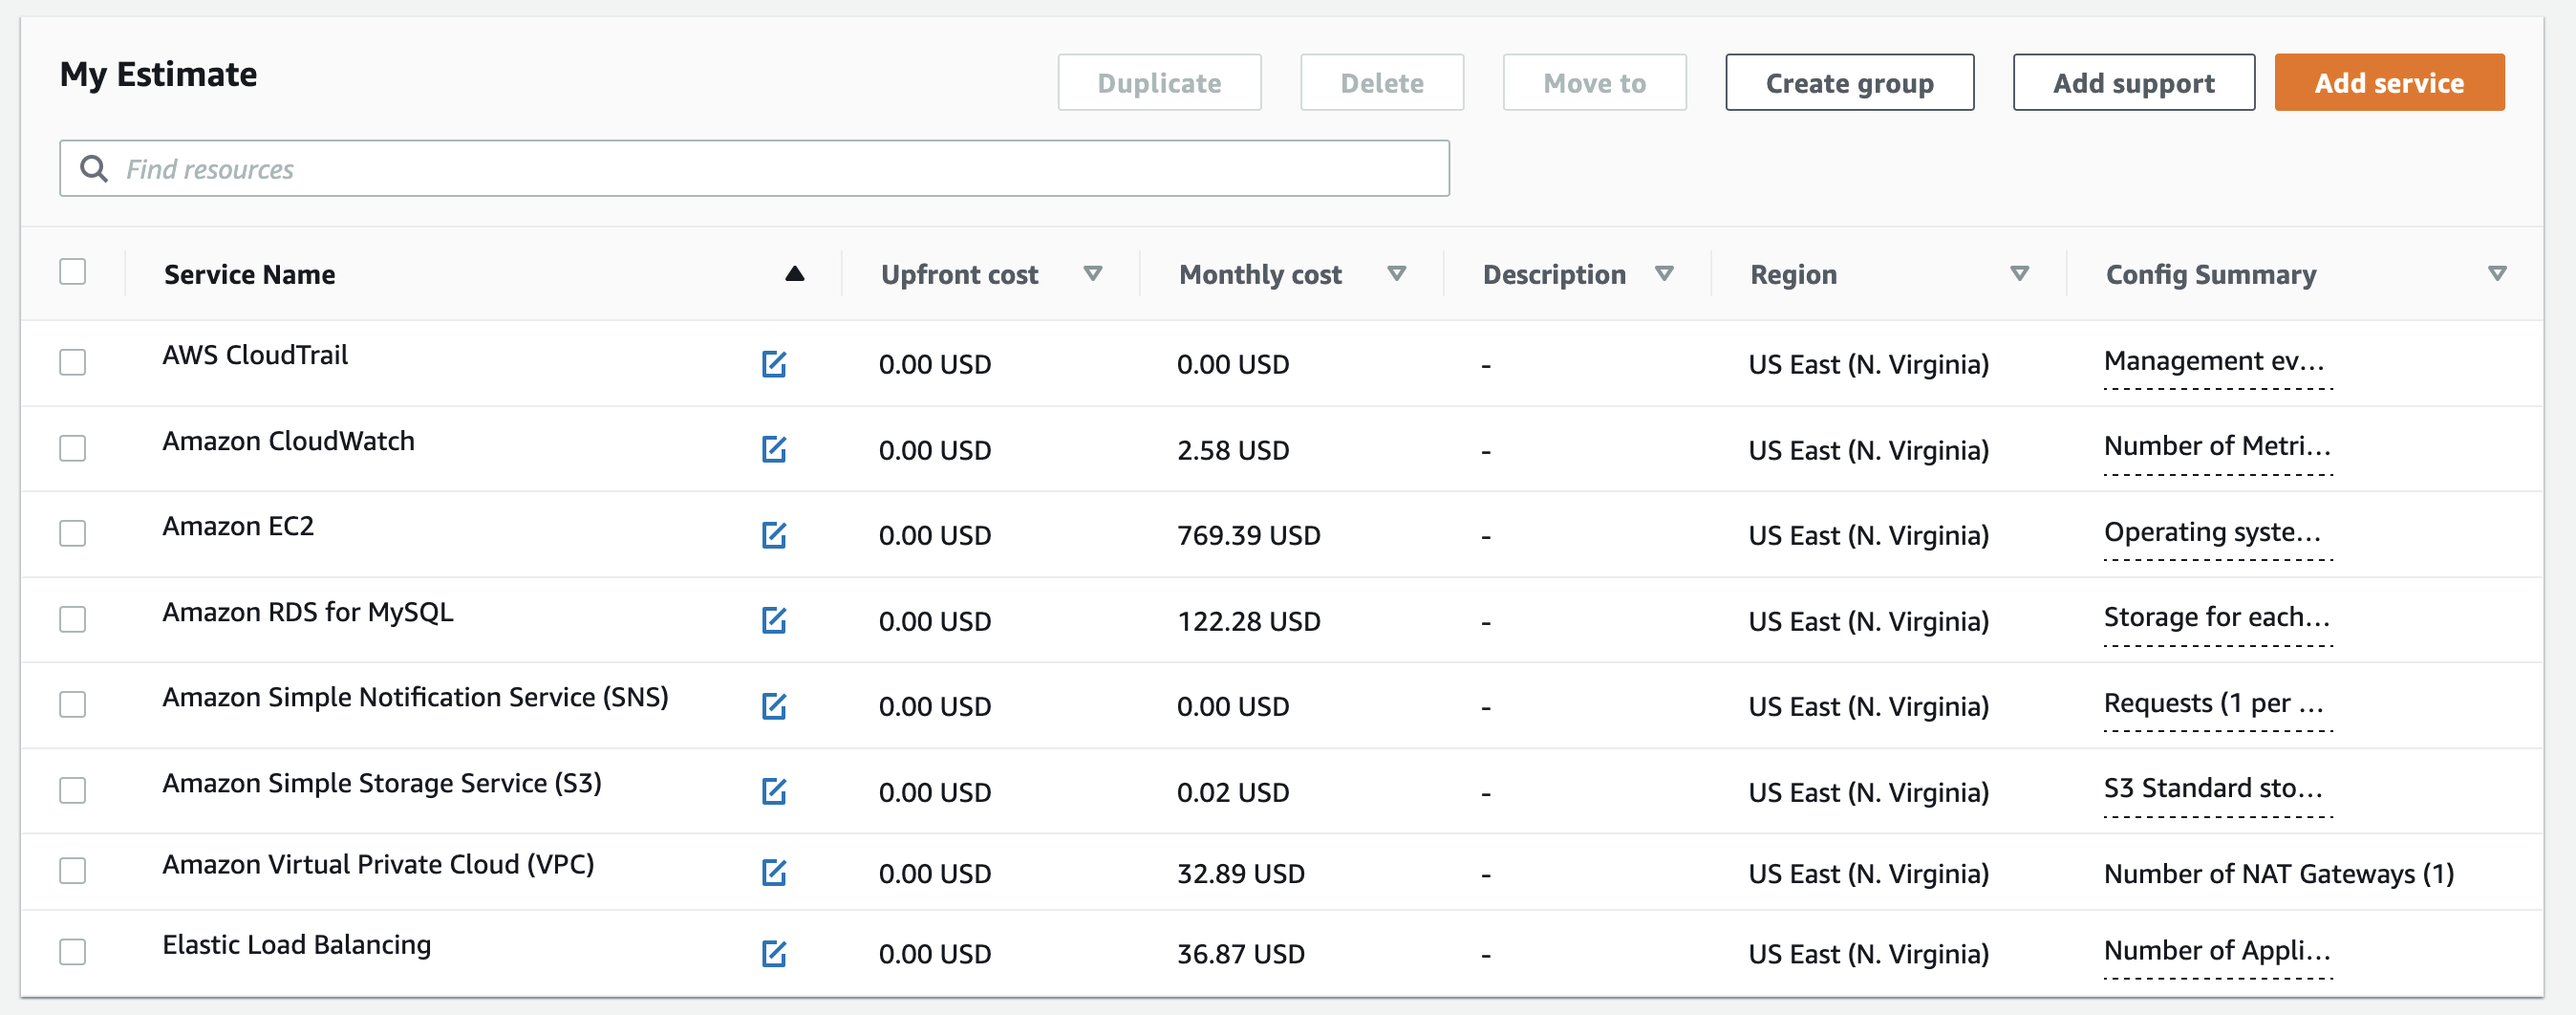
\includegraphics[width=150mm]{resources/cost/scaling-1-million-2}}
    \caption{Estimated cost for scaling up to 1 million users.}
    \label{fig:1-million-users}
\end{figure}

\clearpage
\section{Scaling Up to 10 Million Users}\label{sec:scaling-up-to-10-million-users}
Finally, to scale the application up to 10 million users, the total number of EC2 instances was doubled and the
instance type was kept the same for each.
With each instance providing 16 GB of RAM, the total memory is increased to 320 GB\@.
As more users will be viewing and editing more stories more frequently, the RDS instance type was changed to
\mintinline{zsh}|db.t3.large|, which grants an additional 4 GB of RAM\@.
Additionally, the storage was doubled to 200 GB\@.
This scaling would increase the cost of maintaining the web app to 2064.22 USD per month or 24,770.96 USD per year.

\begin{figure}[!htbp]
    \centering
    \subfloat{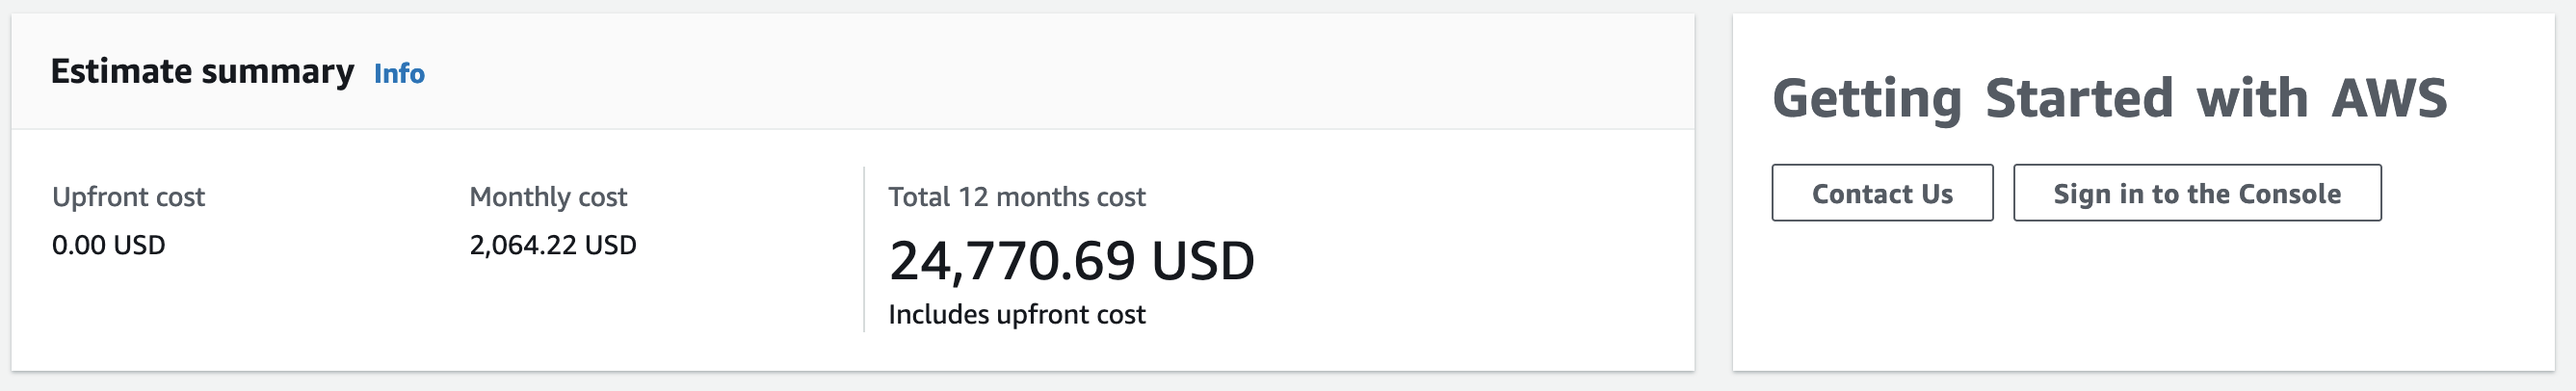
\includegraphics[width=150mm]{resources/cost/scaling-10-million-1}}\hfill
    \subfloat{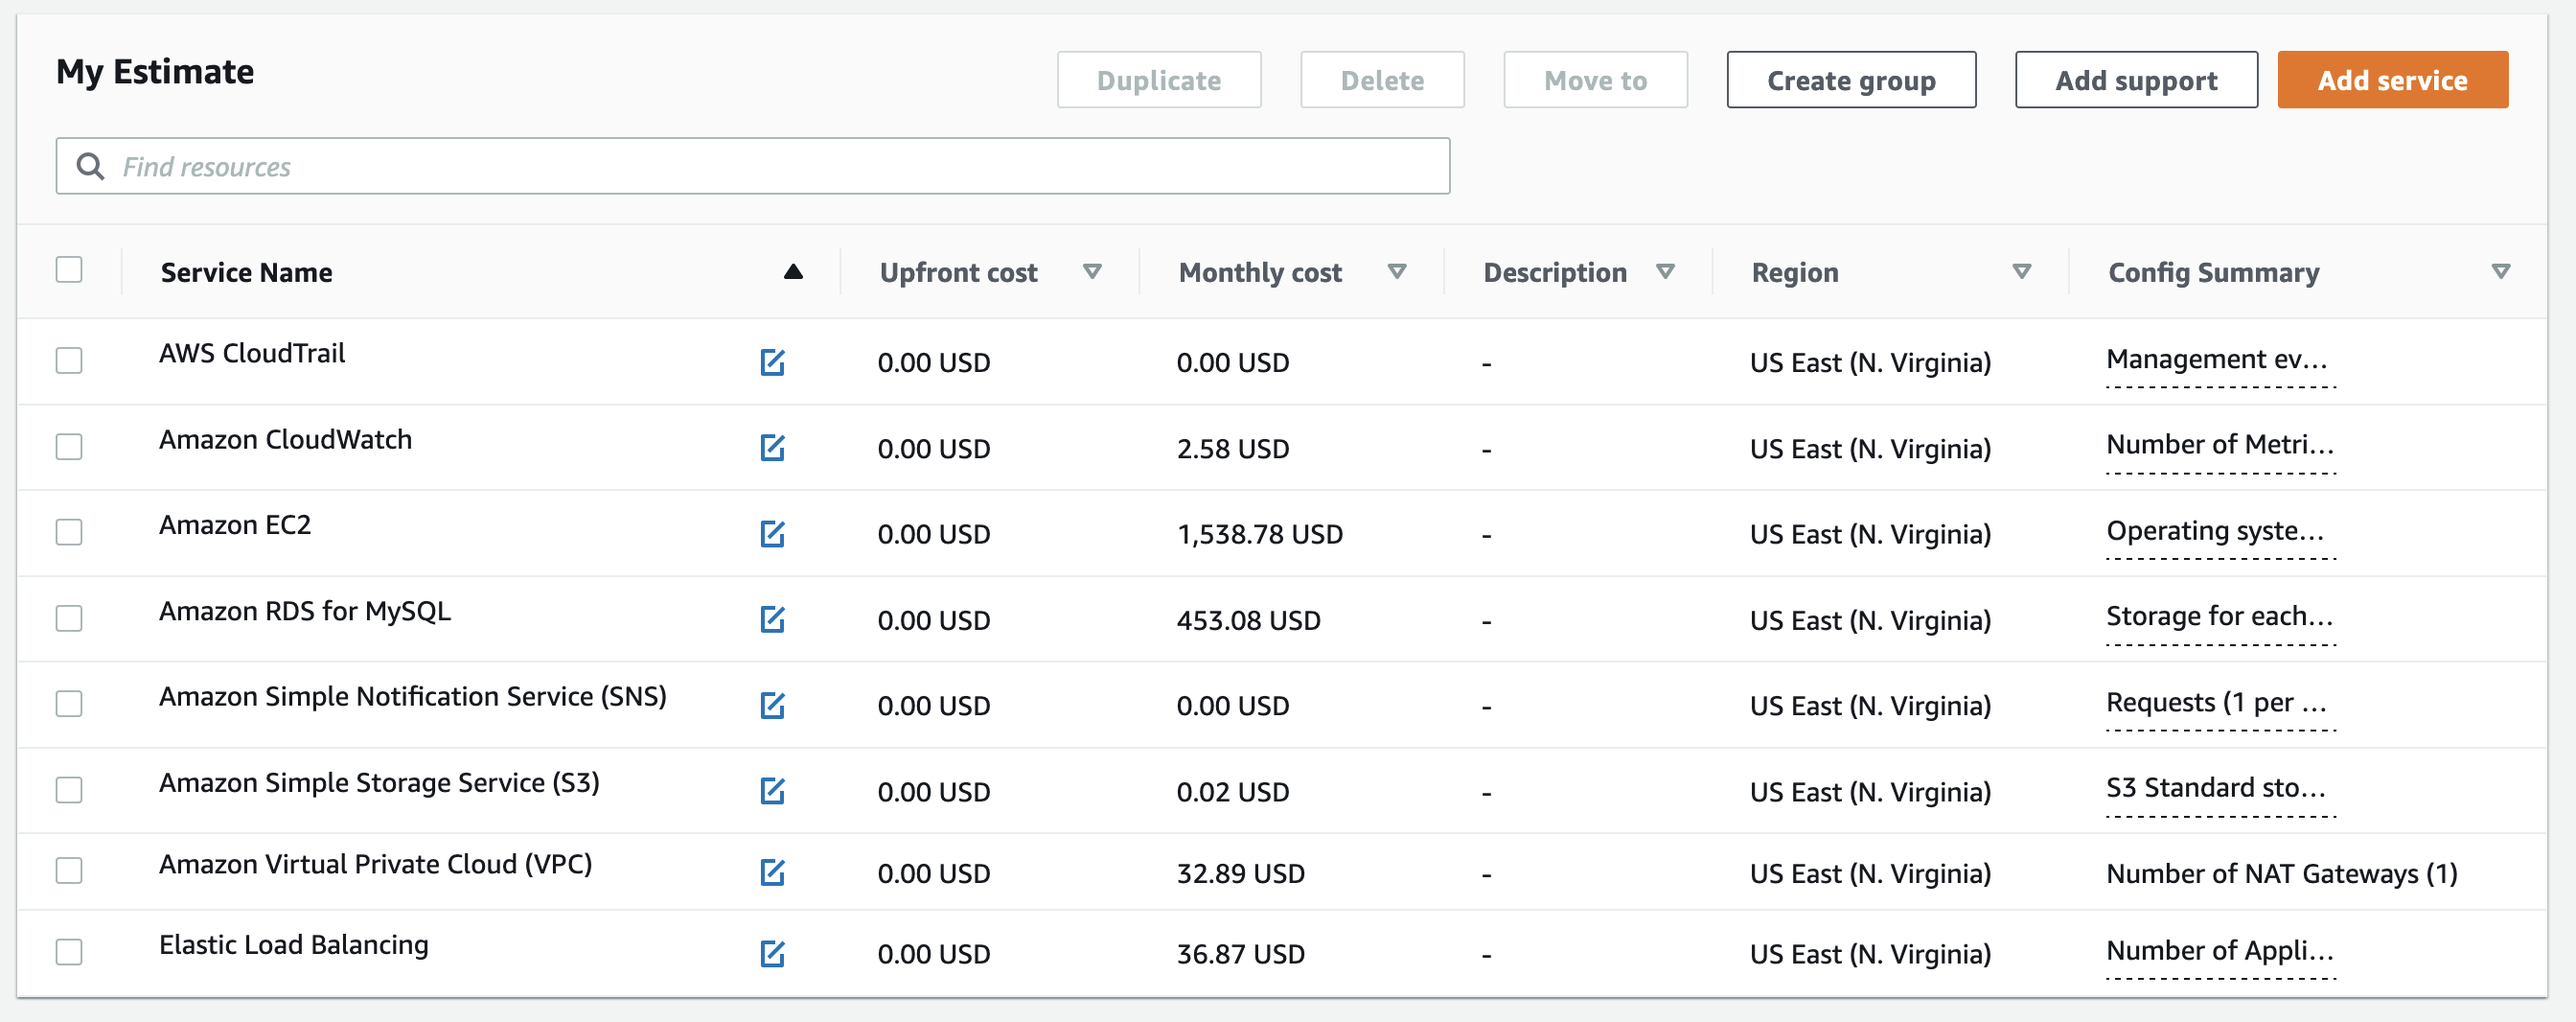
\includegraphics[width=150mm]{resources/cost/scaling-10-million-2}}
    \caption{Estimated cost for scaling up to 10 million users.}
    \label{fig:10-million-users}
\end{figure}

\clearpage
\section{Estimated Costs}\label{sec:estimated-costs}

A summarised breakdown of the monthly cost of maintaining the web app deployment is detailed in Table~\ref{fig:aaaa}.

\begin{table}[!htbp]
    \centering
    \begin{tabular}{|>{\hspace{0pt}}m{0.177\linewidth}|>{\RaggedLeft\hspace{0pt}}m{0.155\linewidth}|>{\RaggedLeft\hspace{0pt}}m{0.198\linewidth}|>{\RaggedLeft\hspace{0pt}}m{0.2\linewidth}|>{\RaggedLeft\hspace{0pt}}m{0.2\linewidth}|}
        \hline
        \multicolumn{5}{|>{\Centering\hspace{0pt}}m{0.929\linewidth}|}{{\cellcolor[rgb]{0.6,0.6,0.6}}\textbf{Monthly Cost Predictions (USD) }} \\
        \hline
        \rowcolor[rgb]{0.8,0.8,0.8} \multicolumn{1}{|>{\Centering\hspace{0pt}}m{0.177\linewidth}|}{\textbf{Feature}} & \multicolumn{1}{>{\Centering\hspace{0pt}}m{0.155\linewidth}|}{\textbf{Cost for }\par{}\textbf{100 Users}} & \multicolumn{1}{>{\Centering\hspace{0pt}}m{0.198\linewidth}|}{\textbf{Cost for }\par{}\textbf{10,000 Users}} & \multicolumn{1}{>{\Centering\hspace{0pt}}m{0.2\linewidth}|}{\textbf{Cost for 1 }\par{}\textbf{million users}} & \multicolumn{1}{>{\Centering\hspace{0pt}}m{0.2\linewidth}|}{\textbf{Cost for 10 }\par{}\textbf{million users}} \\
        \hline
        CloudTrail & 0.01 & 0.01 & 0.01 & 0.01 \\
        \hline
        CloudWatch & 0.80 & 2.58 & 2.58 & 2.58 \\
        \hline
        EC2 & 12.11 & 108.75 & 769.39 & 1,538.78 \\
        \hline
        RDS & 31.72 & 40.92 & 122.28 & 453.08 \\
        \hline
        SNS & \textless{} 0.01 & 0.01 & 0.01 & 0.01 \\
        \hline
        S3 & 0.02 & 0.02 & 0.02 & 0.02 \\
        \hline
        VPC & 31.03 & 32.89 & 32.89 & 32.89 \\
        \hline
        ELB & 36.87 & 36.87 & 36.87 & 36.87 \\
        \hline
        \rowcolor[rgb]{0.6,0.6,0.6} \multicolumn{1}{|>{\RaggedLeft\hspace{0pt}}m{0.177\linewidth}|}{\textbf{Total}} & 112.55 & 222.03 & 964.03 & 2,064.22 \\
        \hline
    \end{tabular}
    \caption{Monthly Cost Predictions.}
    \label{fig:aaaa}
\end{table}

A summarised breakdown of the annual cost of maintaining the web app deployment is detailed in Table~\ref{fig:eeee}.

\begin{table}[!htbp]
    \centering
    \begin{tabular}{|>{\hspace{0pt}}m{0.177\linewidth}|>{\RaggedLeft\hspace{0pt}}m{0.155\linewidth}|>{\RaggedLeft\hspace{0pt}}m{0.198\linewidth}|>{\RaggedLeft\hspace{0pt}}m{0.2\linewidth}|>{\RaggedLeft\hspace{0pt}}m{0.2\linewidth}|}
        \hline
        \multicolumn{5}{|>{\Centering\hspace{0pt}}m{0.929\linewidth}|}{{\cellcolor[rgb]{0.6,0.6,0.6}}\textbf{~Annual Cost Predictions (USD) }} \\
        \hline
        \rowcolor[rgb]{0.8,0.8,0.8} \multicolumn{1}{|>{\Centering\hspace{0pt}}m{0.177\linewidth}|}{\textbf{Feature}} & \multicolumn{1}{>{\Centering\hspace{0pt}}m{0.155\linewidth}|}{\textbf{Cost for }\par{}\textbf{100 Users}} & \multicolumn{1}{>{\Centering\hspace{0pt}}m{0.198\linewidth}|}{\textbf{Cost for }\par{}\textbf{10,000 Users}} & \multicolumn{1}{>{\Centering\hspace{0pt}}m{0.2\linewidth}|}{\textbf{Cost for 1 }\par{}\textbf{million users}} & \multicolumn{1}{>{\Centering\hspace{0pt}}m{0.2\linewidth}|}{\textbf{Cost for 10 }\par{}\textbf{million users}} \\
        \hline
        CloudTrail & \textless{} 0.01 & 0.01 & 0.01 & 0.01 \\
        \hline
        CloudWatch & 9.60 & 30.96 & 30.96 & 30.96 \\
        \hline
        EC2 & 145.32 & 1,305.00 & 9,232.68 & 18,465.36 \\
        \hline
        RDS & 380.64 & 491.04 & 1,467.36 & 5,436.96 \\
        \hline
        SNS & 0.01 & 0.01 & 0.01 & 0.01 \\
        \hline
        S3 & 0.24 & 0.24 & 0.24 & 0.24 \\
        \hline
        VPC & 372.36 & 394.68 & 394.68 & 394.68 \\
        \hline
        ELB & 442.44 & 442.44 & 442.44 & 442.44 \\
        \hline
        \rowcolor[rgb]{0.6,0.6,0.6} \multicolumn{1}{|>{\RaggedLeft\hspace{0pt}}m{0.177\linewidth}|}{\textbf{Total}} & 1,350.6 & 2,664.36 & 11,568.36 & 24,770.64 \\
        \hline
    \end{tabular}
    \caption{Annual Cost Predictions.}
    \label{fig:eeee}
\end{table}
